\section{Presencial laboratory}
\label{sec:Presencial}

In this last laboratory assigment, due to some changes in the university directives, one student from each group was allowed to participate in a laboratory session presencialy. This change was very positive beacause although we could simulate and learn from our experiences in the Ngspice software, being able to see and feel the components brings another meaning and perspective to the work we have been doing throughout the semester and motivates the students to explore and persue careers in the eletronics field.Therefore we thank the professor for the time it took to make thsi labs possible and for sparking our curiosity for this field. Here are some of the pictures we were able to take during the lab assigment:  

\begin{figure}[H] \centering
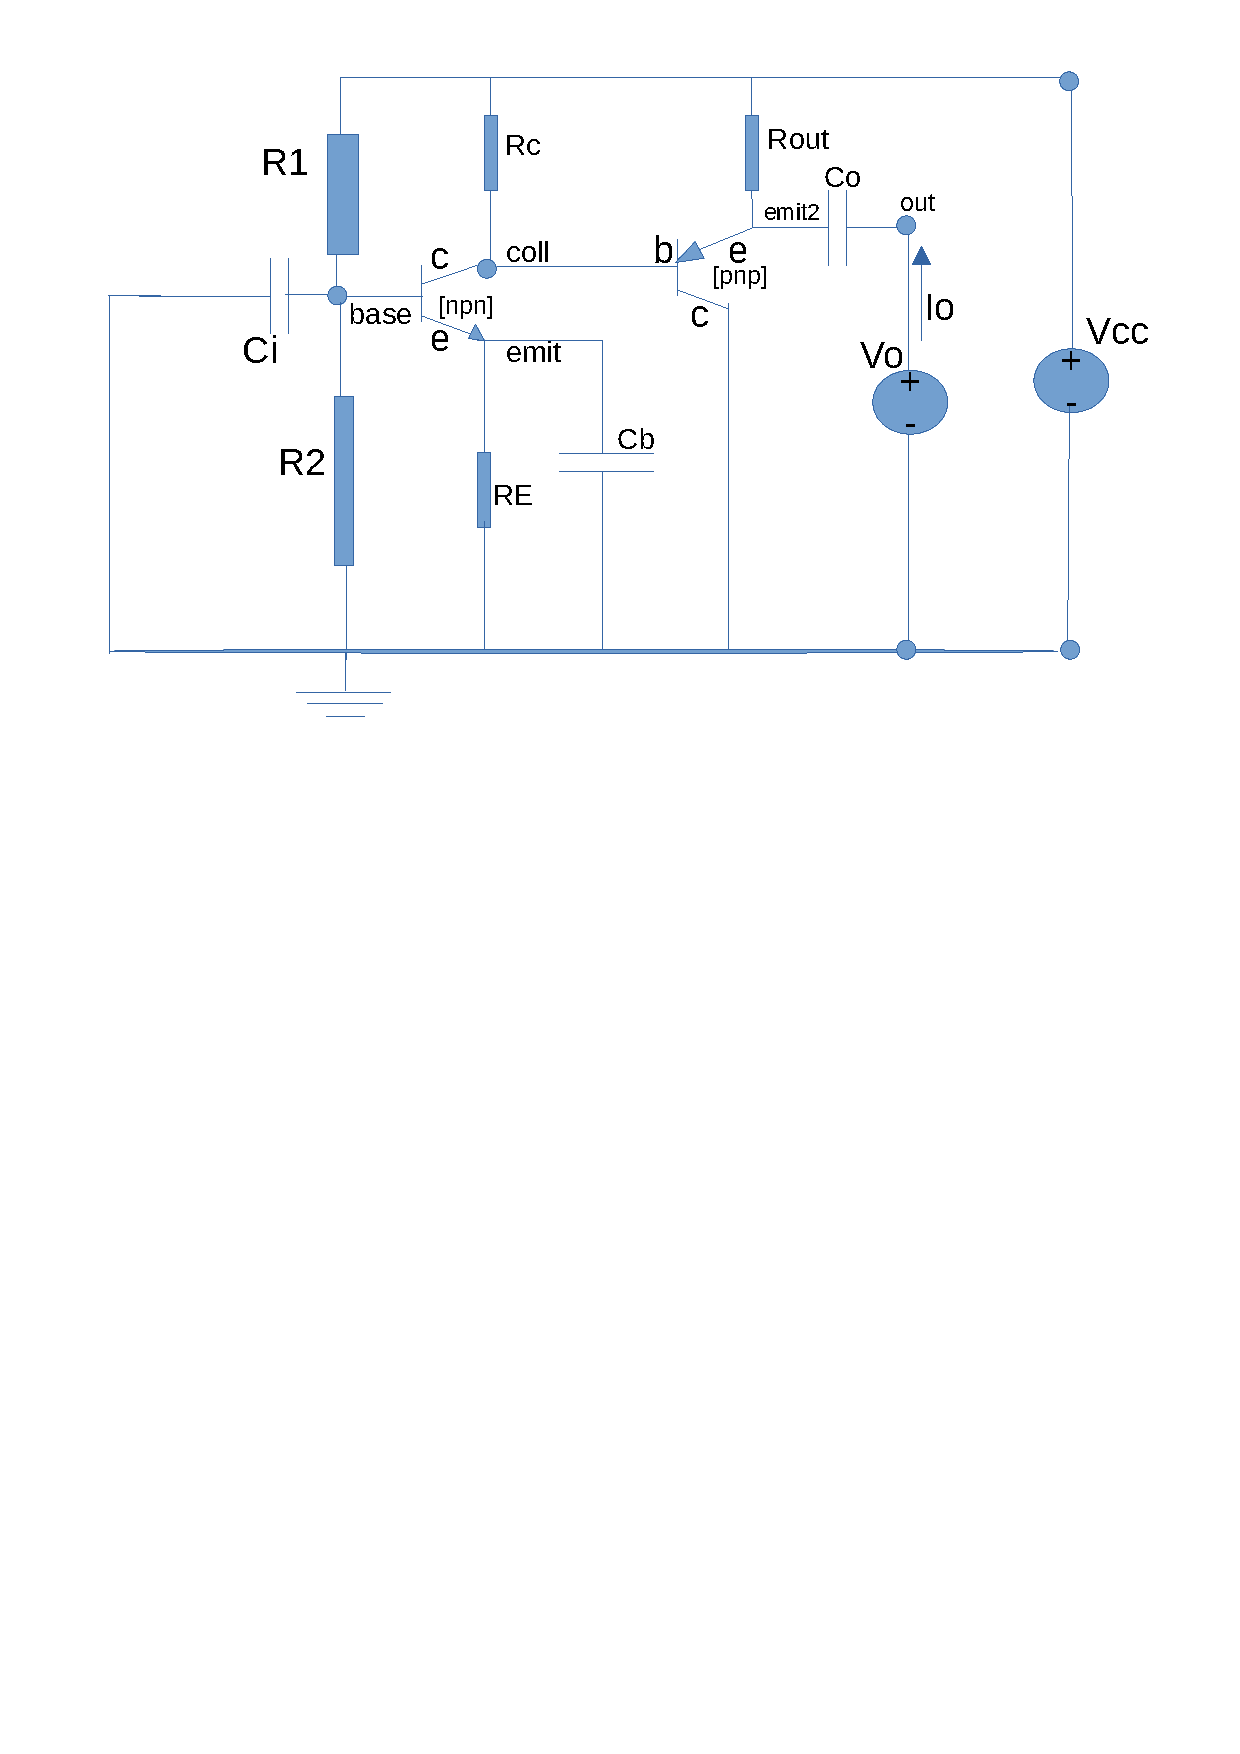
\includegraphics[width=0.95\linewidth]{diagram_t4_zout.pdf}
\vspace{-10cm}
\caption{Diagram of the circuit considered for the simulation of the output impedance of the amplifier .}
\label{fig:diagram_t4_zout}
\end{figure}

  
\begin{figure}[H] \centering
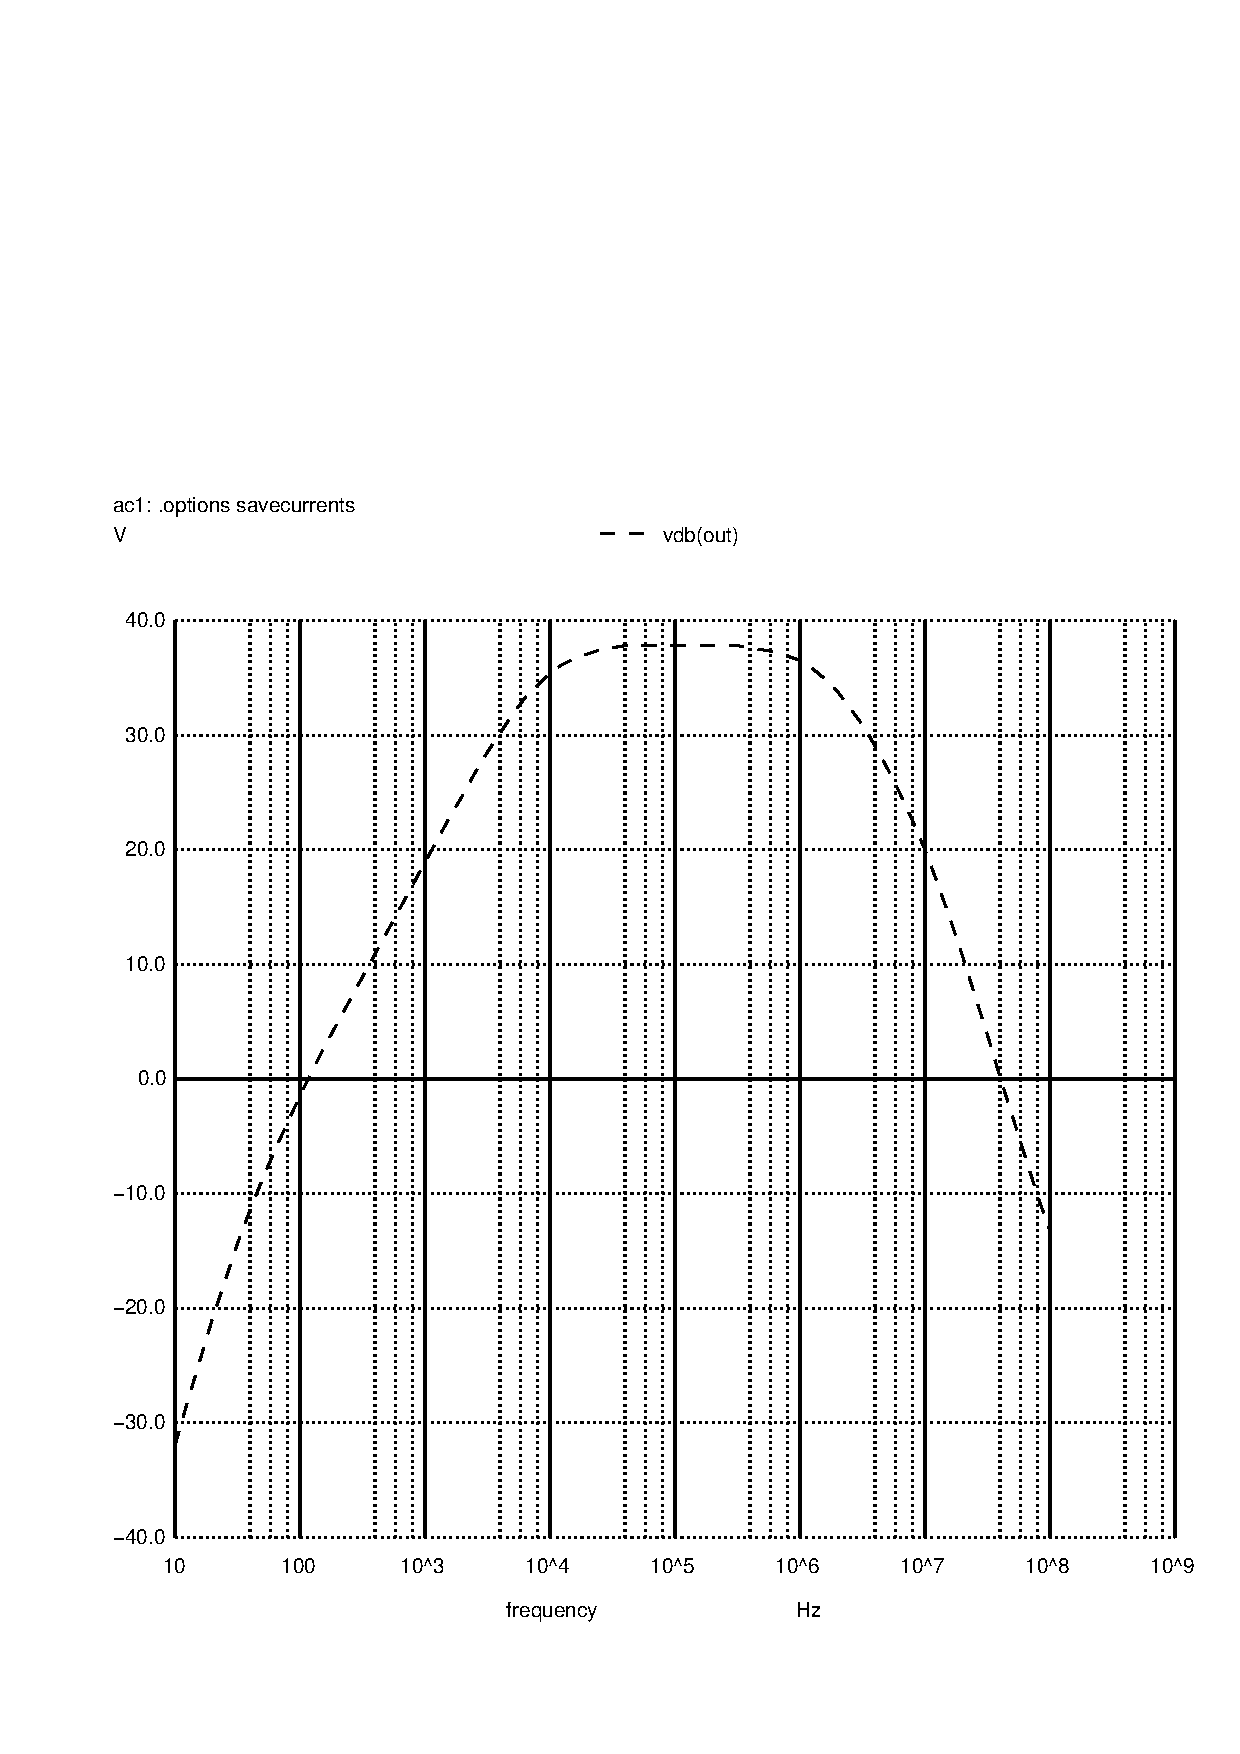
\includegraphics[width=0.6\linewidth]{vo2f.pdf}
\vspace{-1cm}
\caption{Output voltage gain in the passband}
\label{fig:gain_sim}
\end{figure}


\begin{figure}[H] \centering
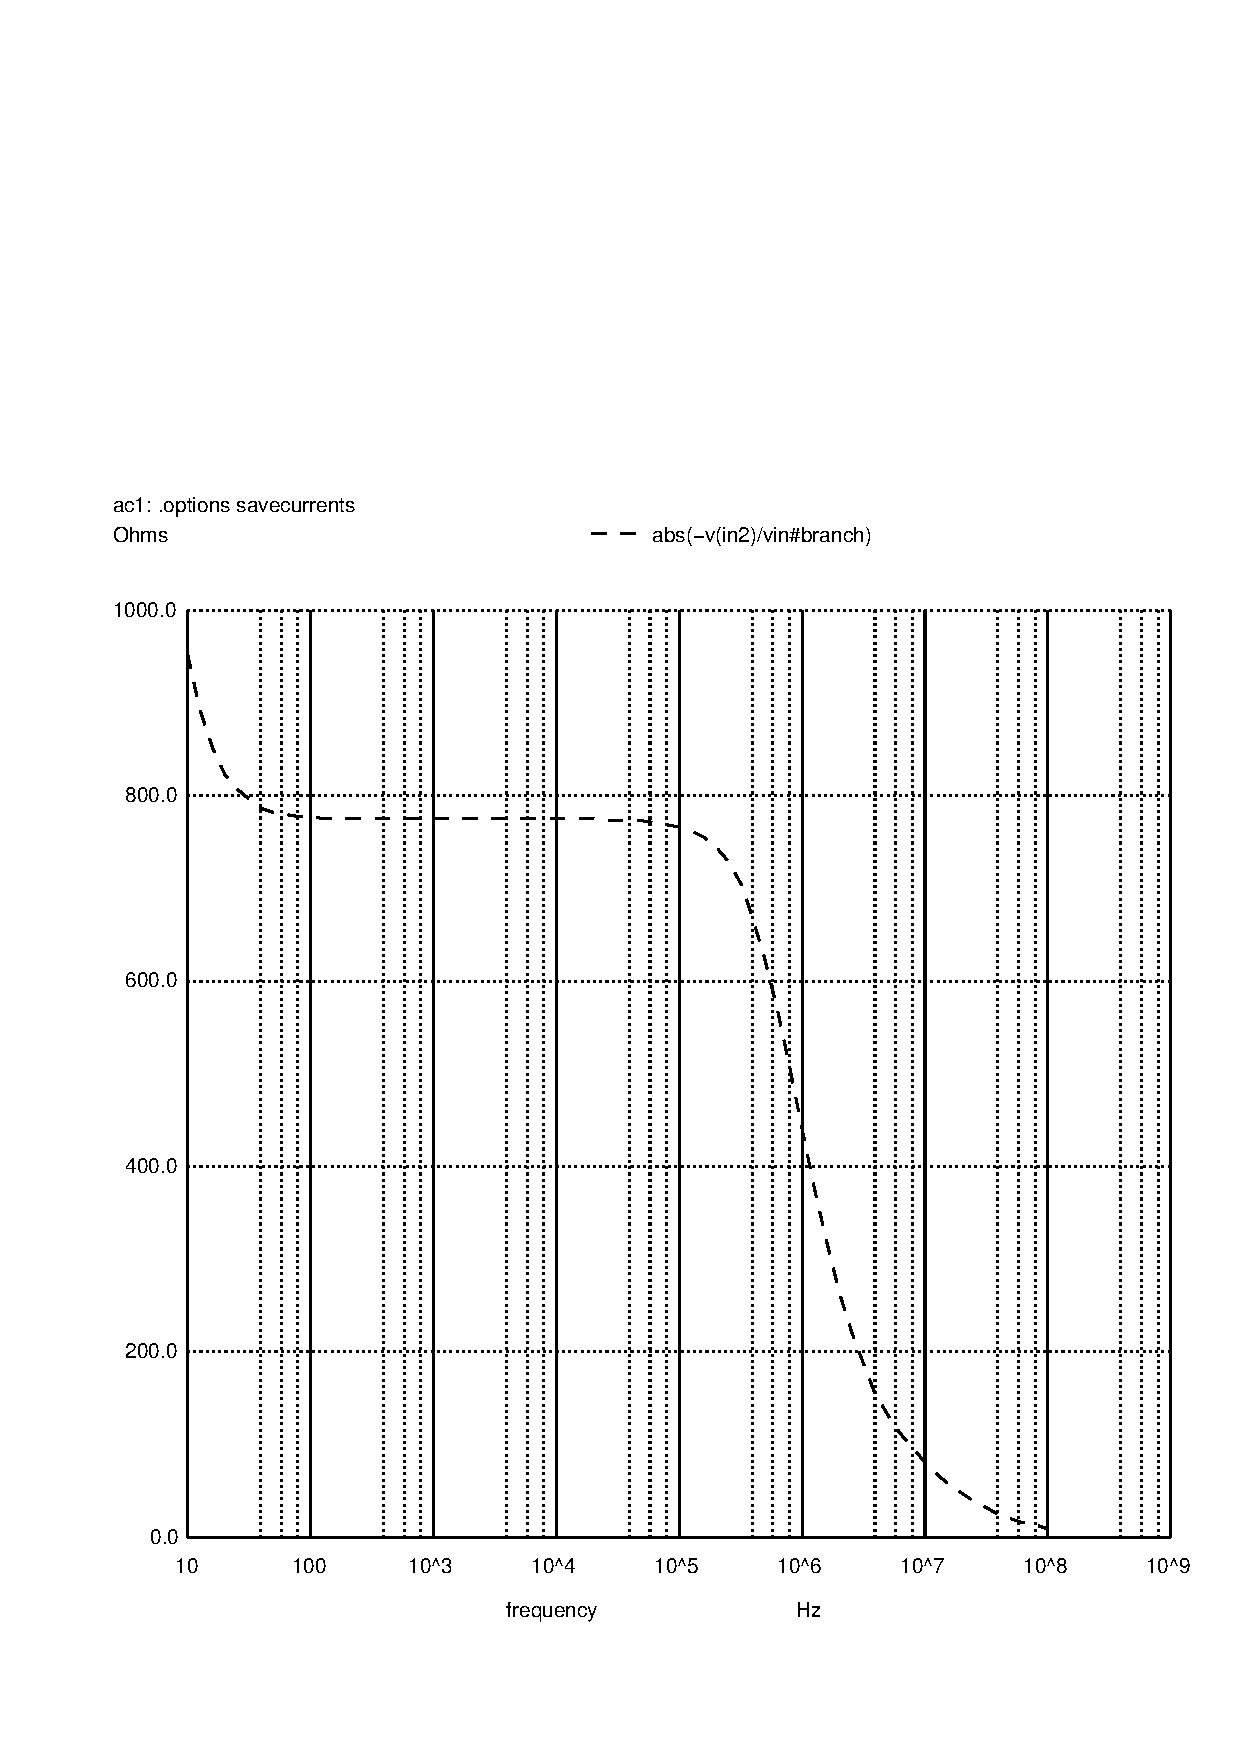
\includegraphics[width=0.6\linewidth]{zin.pdf}
\caption{Input impedance of the Audio amplifier circuit}
\label{fig:In_imp}
\end{figure}
\vspace{-3cm}


\begin{figure}[H] \centering
\includegraphics[width=0.6\linewidth]{zoinc.pdf}
\caption{Output impedance of the Audio amplifier circuit}
\label{fig:out_imp}
\end{figure}
\vspace{-3cm}


\pagebreak
